\documentclass[reprint,onecolumn,%endfloats*,
amsmath,amssymb,aip,apl]{revtex4-1}

\usepackage{graphicx}% Include figure files
\usepackage{dcolumn}% Align table columns on decimal point
\usepackage{bm}% bold math
\usepackage{hyperref}% add hypertext capabilities
\usepackage{comment}
\usepackage[version=4]{mhchem}
\usepackage{color}

%\usepackage{float}

\usepackage{siunitx}
\DeclareSIPostPower\tothefourth{4}
\usepackage[english]{babel}
\usepackage{esdiff} % for differentiation

\begin{document}
	\title{RCSJ model using python3}
	\author{Felix E. Schmidt}
	\author{Mark D. Jenkins}
	\affiliation{Kavli Institute of NanoScience, Delft University of Technology, Lorentzweg 1, 2628 CJ, Delft, The Netherlands.}	
	\date{\today}

	\begin{abstract}
		This script is based on Tinkham's "Introduction to superconductivity"\cite{tinkham} and Gross' "Applied superconductivity", chapter 3 \cite{gross}.
		All simulations were done using \texttt{python3} and the \texttt{rcsj} module written by Felix \cite{rcsj}.
	\end{abstract}	
	
	\maketitle
	\tableofcontents
	
	
	\section{Current biasing}
	\subsection{Junction model and ODE}
	We model the Josephson junction in the simplest way possible:
	A series network of a resistor $R$, a capacitor $C$ and a nonlinear inductor.
	The total current running through the network is
	\begin{eqnarray}
	I(t) =& I_s(t) + I_R(t) + I_C(t) \\%
	I(t) =& I_c\sin(\phi) + \frac{V}{R} + C\diff{V}{t} \\%
	V(t) =& \frac{\hbar}{2e}\diff{\phi}{t}, \; \diff{V}{t} = \frac{\hbar}{2e} \diff[2]{\phi}{t} \\%
	\rightarrow I(t) =& I_c\sin(\phi)+\frac{\hbar}{2eR}\diff{\phi}{t}+\frac{\hbar C}{2e}\diff[2]{\phi}{t}
	\end{eqnarray}
	There are two approaches to simplifying this equation in terms of normalization.
	We here call them the \textbf{Tinkham approach}\cite{tinkham} and the \textbf{Gross approach}\cite{gross}.
	
	
	\subsubsection{Tinkham approach}
	The equation is simplified with normalized time via the plasma frequency, $\tau=\omega_p t$:
	\begin{eqnarray}
	\omega_p=\frac{1}{\tau_p}=\frac{1}{\sqrt{L_c C}}=\sqrt{\frac{2eI_c}{\hbar C}} \\%
	{\rm d}t=\frac{1}{\omega_p}{\rm d}\tau \rightarrow \diff[n]{}{t}=\omega_p^n \diff[n]{}{\tau} \\%
	\frac{I}{I_c}-\sin(\phi) = \underbrace{\frac{\hbar}{2eI_cR}\sqrt{\frac{2eI_c}{\hbar C}}}_{\sqrt{\frac{\hbar C}{2eI_c}}\frac{1}{RC}\equiv Q^{-1}}\diff{\phi}{\tau}+\underbrace{\frac{\hbar C}{2eI_c}\frac{2eI_c}{\hbar C}}_{1}\diff[2]{\phi}{\tau}
	\end{eqnarray}
	Hence the final ODE is
	\begin{eqnarray}
	\diff[2]{\phi}{\tau}=\frac{I}{I_c}-\sin(\phi)-\frac{1}{Q}\diff{\phi}{\tau}
	\label{eq:tinkham}
	\end{eqnarray}
	
	\subsubsection{Gross approach}
	This approach is different in that it seems more intuitive, but the time scale and damping are different:
	We normalize the time not by the plasma frequency, but the $L_c/R_n$ time constant that yields the characteristic junction frequency:
	\begin{eqnarray}
	\omega_c=\frac{1}{\tau_c}=\frac{R_n}{L_c}=\frac{2e}{\hbar}I_cR_n=\frac{\Phi_0}{2\pi}V_c \\%
	\tau=\frac{t}{\tau_c}, \; \tau_c=\frac{\hbar}{2e I_cR} \\%
	{\rm d}t=\tau_c{\rm d}\tau \rightarrow \diff[n]{}{t}=\frac{1}{\tau_c^{n}}\diff[n]{}{\tau}
	\end{eqnarray}
	The above ODE then can be resorted into
	\begin{eqnarray}
	I-I_c\sin(\phi)=\frac{\hbar\tau_c}{2eR}\diff{\phi}{\tau}+\frac{\hbar C \tau^2}{2e}\diff[2]{\phi}{\tau} \\%
	i-\sin(\phi)=\underbrace{\frac{\hbar}{2eRI_c}\left(\frac{2eI_cR}{\hbar}\right)}_{1}\diff{\phi}{\tau}+\underbrace{\frac{\hbar C}{2e}\left(\frac{2eI_cR}{\hbar}\right)^2}_{\frac{2eI_cR^2C}{\hbar}=\beta_c} \diff[2]{\phi}{\tau} \\%
	\diff[2]{\phi}{\tau} = \frac{1}{\beta_c}\left(i-\sin(\phi)-\diff{\phi}{\tau}\right)
	\label{eq:gross}
	\end{eqnarray}
	Note that $\beta_c\equiv Q^2\equiv\tau_c RC$.
	For this ODE it is much easier to distinguish between $\beta_c\gg1$ and $\beta_c\ll1$, simply because of its form.
	However, it is important to keep in mind that the timescales are different!
	
	\subsection{Unit discussion}
	We consider first $\tau_c$.
	The units of $\hbar/(2e)=\Phi_0/(2\pi)$ are \si{Wb}=\si{\kilogram\meter\squared\per\second\squared\per\ampere}.
	Critical current is in \si{\ampere}, resistance in \si{\ohm}=\si{\kilogram\meter\squared\per\second\cubed\per\ampere\squared}.
	Therefore
	\begin{eqnarray}
	\left[\tau_c\right]=\left[\frac{\hbar}{2e}\frac{1}{I_c}\frac{1}{R}\right] = \frac{\si{\kilogram\meter\squared}}{\si{\second\squared\ampere}}\frac{1}{\si{\ampere}}\frac{\si{\second\cubed\ampere\squared}}{\si{\kilogram\meter\squared}} = \si{\second} \\%
	\rightarrow \left[\tau\right]=\left[\frac{t}{\tau_c}\right]=\frac{\si{\second}}{\si{\second}}=1
	\end{eqnarray}
	Now the same for the plasma frequency:
	Capacitance is given in units of \si{F}=\si{\second\tothefourth\ampere\squared\per\meter\squared\per\kilogram}
	\begin{eqnarray}
	\left[\omega_p\right]=\left[\sqrt{\frac{2e}{\hbar}\frac{I_c}{C}}\right]=\sqrt{\frac{\si{\second\squared\ampere}}{\si{\kilogram\meter\squared}}\si{\ampere}\frac{\si{\meter\squared\kilogram}}{\si{\second\tothefourth\ampere\squared}}}=\sqrt{\frac{1}{\si{\second\squared}}}=\frac{1}{\si{\second}} \\%
	\rightarrow \left[\tau\right]=\left[\omega_p t\right]=\frac{\si{\second}}{\si{\second}}=1
	\end{eqnarray}
	
	\subsection{Damping}
	We consider eq. \ref{eq:gross} for simplicity.
	For \textbf{very weak damping}, i.e. $\beta_c\gg1$, the left hand side of the ODE can be set to zero.
	The result is a linear IVC on the retrapping branch, with $I_r\leq I_c$:
	\begin{eqnarray}
	\diff[2]{\phi}{\tau}=0 \rightarrow \langle V(t)\rangle=IR_n \\%
	\frac{I_r}{I_c}\approx\frac{4}{\pi\sqrt{\beta_c}}\equiv\frac{4}{\pi Q}
	\end{eqnarray}
	An open question is why Gross (and others) report significant hysteresis $I_r/I_c\approx0.85$ already for $\beta_c=1$, while we achieve at least $I_r/I_c=0.95$ for the implemented python simulations.
	
	For \textbf{very strong damping}, i.e. $\beta_c\ll1$, the right hand side of the ODE is zero:
	\begin{eqnarray}
	\diff{\phi}{\tau}=i-\sin(\phi) \rightarrow \langle V(t) \rangle=I_c R\sqrt{\left(I/I_c\right)^2-1}
	\end{eqnarray}
	without hysteresis.
	
	
	\begin{figure}
		\centering
		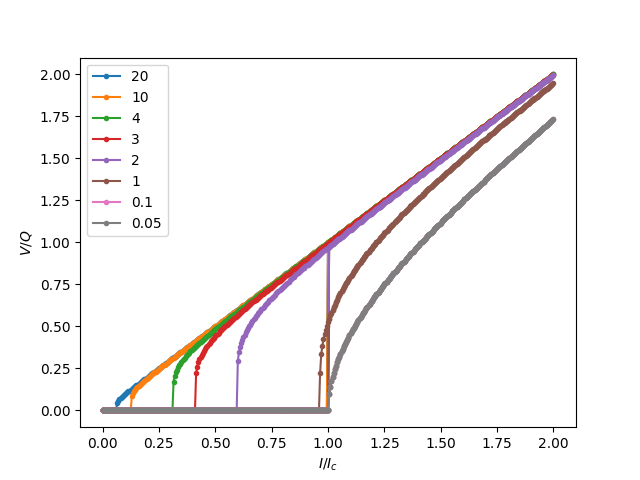
\includegraphics[width=0.5\linewidth]{../plots/ivcs_updown}
		\caption{Current-voltage curves for various damping cases.
			As predicted by theory, high damping ($Q\ll1$) corresponds to a square-root like IVC with no hysteresis, while low damping ($Q\gg1$) results in strong hystersis with a almost linear retrapping branch.}
		\label{fig:ivcsupdown}
	\end{figure}
	
	\subsection{Frequency analysis}
	
	\section{Voltage biasing}
	The system equation only slightly changes.
	What remains to be seen is the normalization and the exact values needed to achieve voltage biasing.
	
	\bibliography{cited.bib}
	
\end{document}
